\documentclass[letterpaper,11pt]{article}
\oddsidemargin -1.0cm \textwidth 17.5cm

\usepackage[utf8]{inputenc}
\usepackage[activeacute,spanish, es-lcroman]{babel}
\decimalpoint
\usepackage{amsfonts,setspace}
\usepackage{amsmath}
\usepackage{amssymb, amsmath, amsthm}
\usepackage{comment}
\usepackage{float}
\usepackage{amssymb}
\usepackage{dsfont}
\usepackage{anysize}
\usepackage{multicol}
\usepackage{enumerate}
\usepackage{graphicx}
\usepackage[left=1.5cm,top=2cm,right=1.5cm, bottom=1.7cm]{geometry}
\setlength\headheight{1.5em} 
\usepackage{fancyhdr}
\usepackage{multicol}
\usepackage{hyperref}
\usepackage{wrapfig}
\usepackage{subcaption}
\usepackage{siunitx}
\usepackage{cancel}
\usepackage{mdwlist}
\usepackage{svg}
\pagestyle{fancy}
\fancyhf{}
\renewcommand{\labelenumi}{\normalsize\bfseries P\arabic{enumi}.}
\renewcommand{\labelenumii}{\normalsize\bfseries (\alph{enumii})}
\renewcommand{\labelenumiii}{\normalsize\bfseries \roman{enumiii})}


\begin{document}

\fancyhead[L]{\itshape{Facultad de Ciencias F\'isicas y Matem\'aticas}}
\fancyhead[R]{\itshape{Universidad de Chile}}
\rfoot[]{pág. \thepage}

\begin{minipage}{11.5cm}
    \begin{flushleft}
        \hspace*{-0.6cm}\textbf{FI1000-1 Introducción a la Física Clásica}\\
        \hspace*{-0.6cm}\textbf{Profesor:} Ignacio Bordeu\\
        \hspace*{-0.6cm}\textbf{Auxiliares:} Alejandro Cartes \& Simón Yáñez\\
        \hspace*{-0.6cm}\textbf{Ayudante:} Javier Cubillos\\
    \end{flushleft}
\end{minipage}

\begin{picture}(2,3)
    \put(366, 10){
\includegraphics[scale=0.9]{2020-1/Imágenes/logo/dfi-fcfm.pdf}}
\end{picture}

\begin{center}
	\LARGE\textbf{Auxiliar \#13}\\
	\Large{Producto Cruz y Torque}
\end{center}

\vspace{-1cm}
\begin{enumerate}\setlength{\itemsep}{0.4cm}

\item[]

\item
\begin{enumerate}
    \item Dado los vectores $\mathbf{A} = -3\mathbf{\hat{i}} + 4\mathbf{\hat{j}}$ y $\mathbf{B} = 2\mathbf{\hat{i}} + 3\mathbf{\hat{j}}$, determine \textbf{i)} $\mathbf{A}\times\mathbf{B}$ y \textbf{ii)} el ángulo entre $\mathbf{A}$ y $\mathbf{B}$
    
    \item Un estudiante afirma que encontró un vector $\mathbf{A}$ tal que $(2\mathbf{\hat{i}}-3\mathbf{\hat{j}}+4\mathbf{\hat{k}})\times\mathbf{A} = (4\mathbf{\hat{i}} + 3\mathbf{\hat{j}}-\mathbf{\hat{k}})$, ¿usted cree esta afirmación?
\end{enumerate}

\item Considere el objeto de la figura (a) formado por cuatro barras de largo $a$ soldadas entre sí en ángulos rectos. La barra superior posee masa $M$, mientras que las tres restantes poseen masa $m$.

\begin{enumerate}
    \item Determine la posición del centro de masa del objeto en el sistema de coordenadas cartesianas $(x, \, y)$ mostrado en la figura (a)
    
    \item El objeto se cuelga de un clavo sin roce que pasa por uno de sus extremos, como se muestra en la figura (b). Si el objeto se encuentra en equilibrio, determine el ángulo $\theta$
\end{enumerate}

\begin{figure}[H]
    \centering
    \begin{subfigure}[t]{0.4\linewidth}
        \centering
        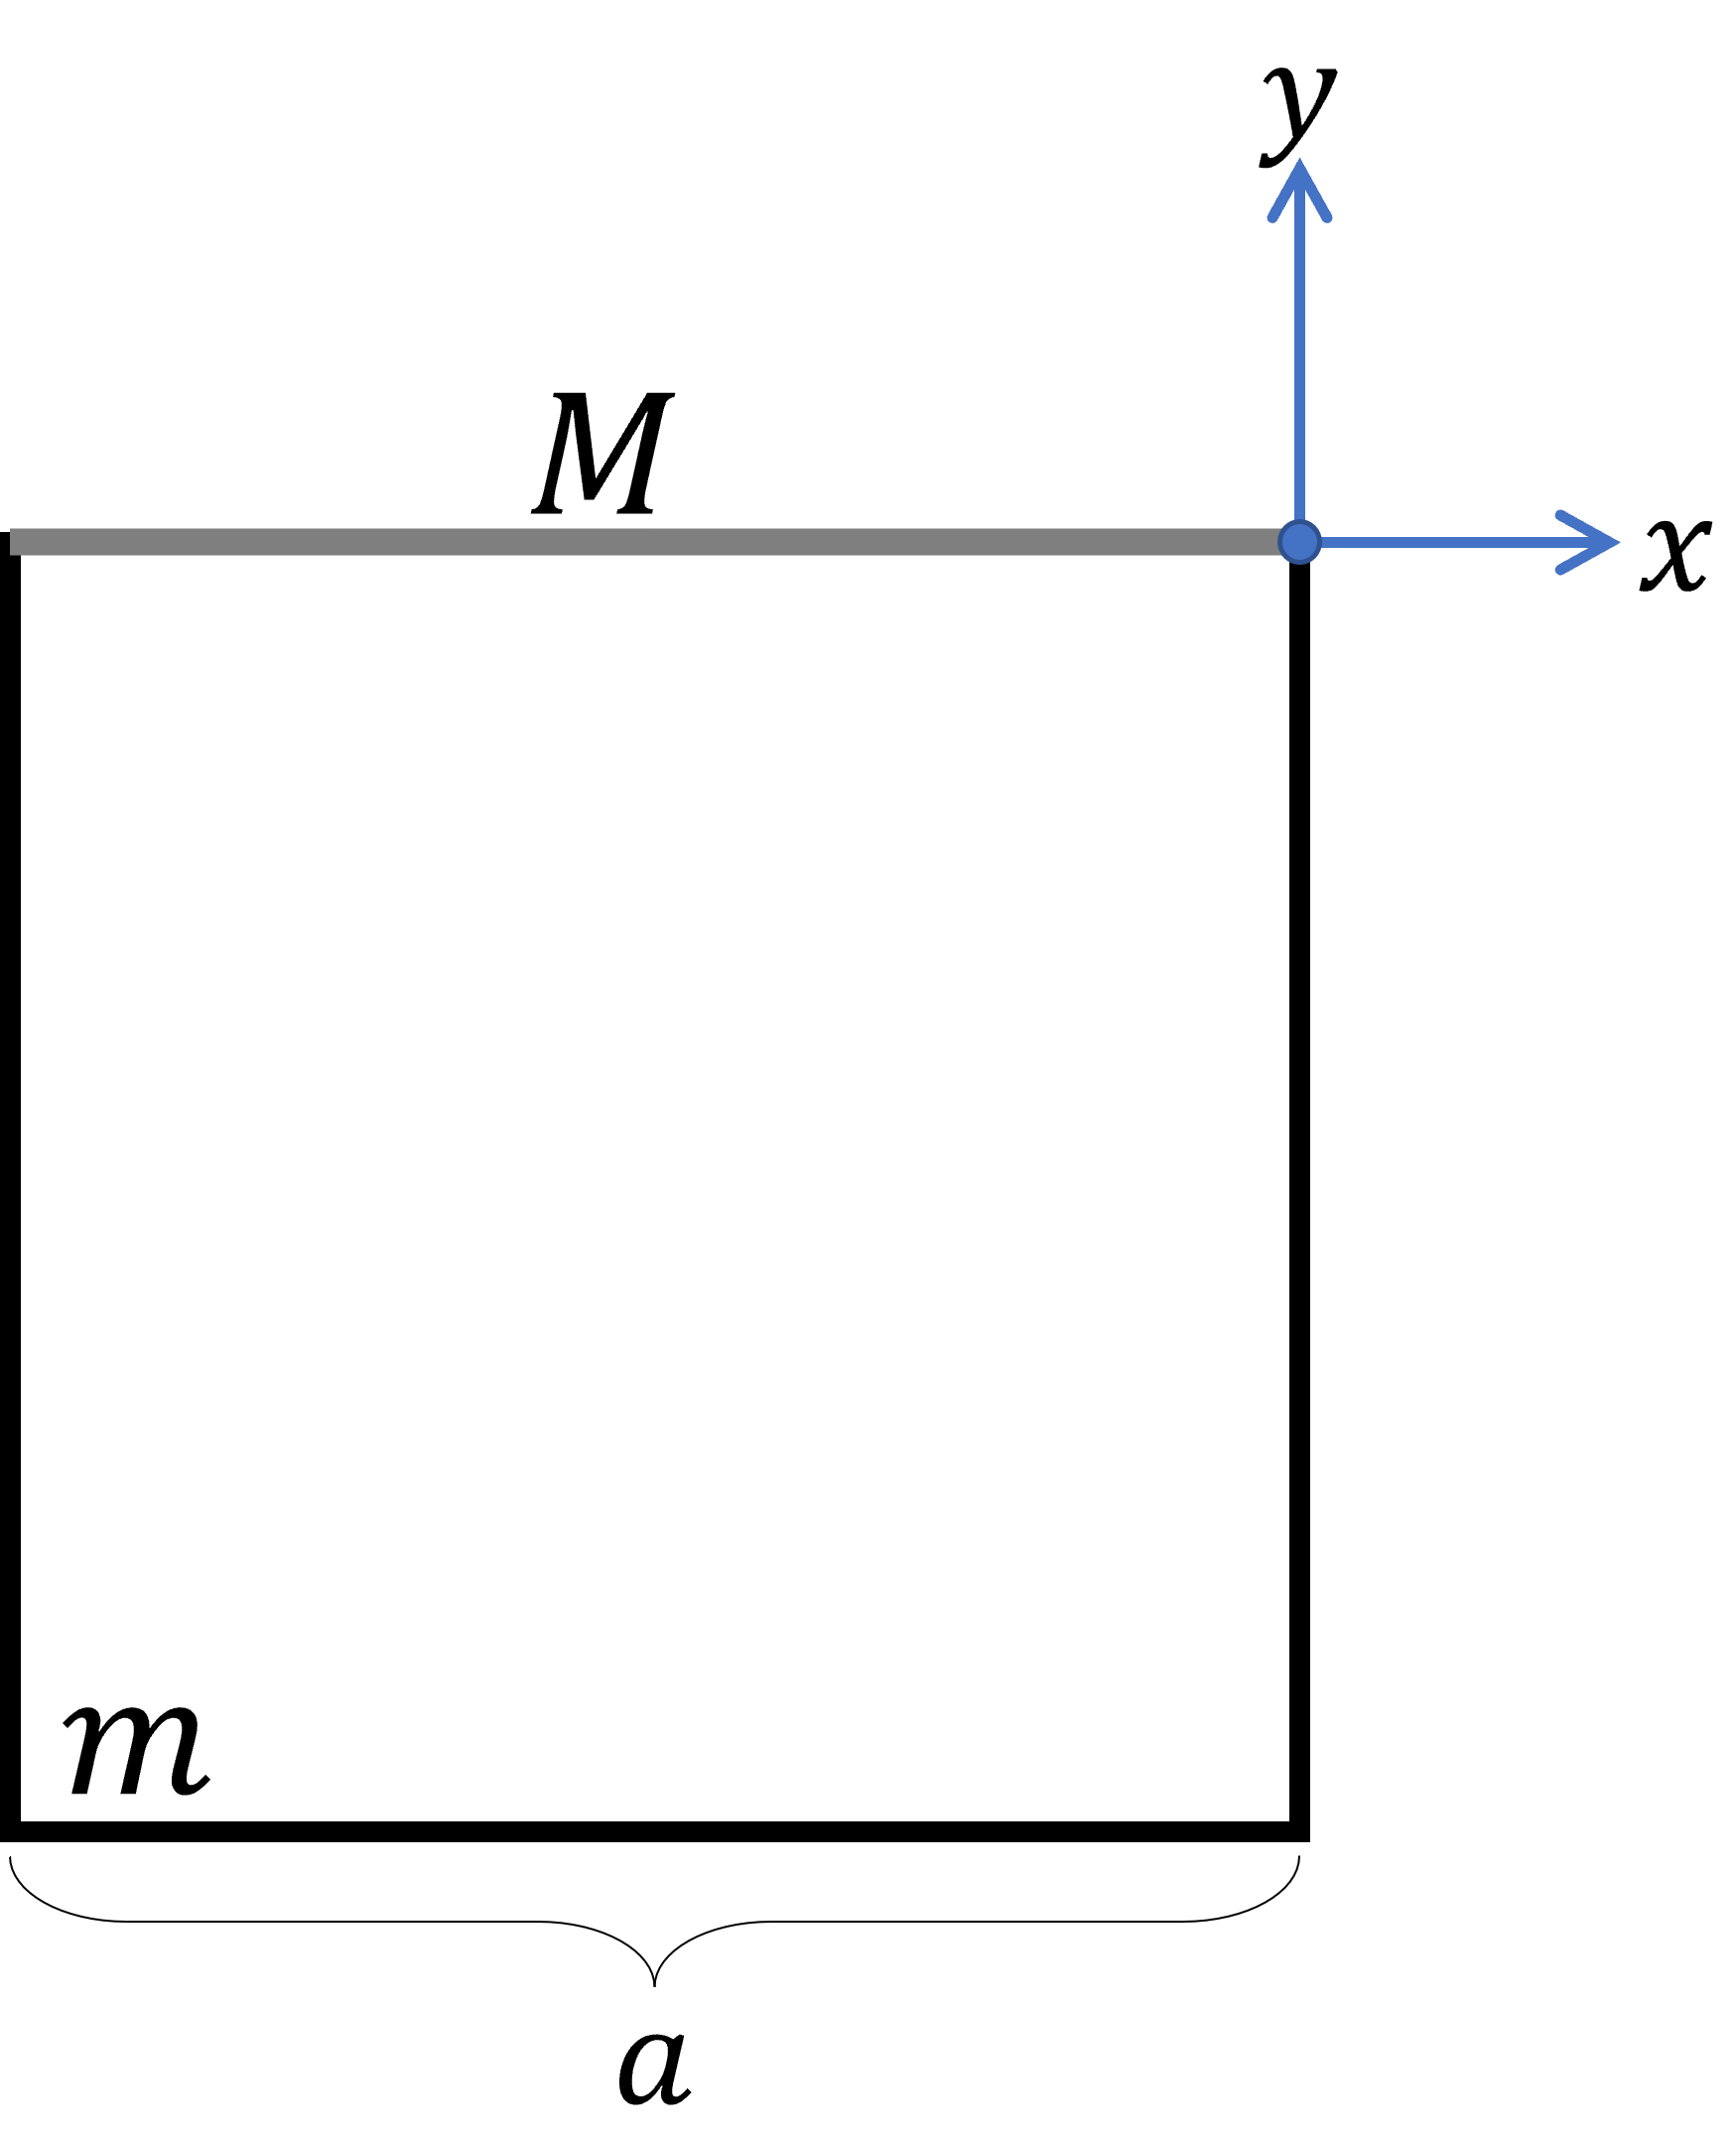
\includegraphics[width=0.7\linewidth]{2022-2/Imagenes/Capsula2/fierro_a.png}
        \caption{}
    \end{subfigure}
    \hspace{3em}
    \begin{subfigure}[t]{0.4\linewidth}
        \centering
        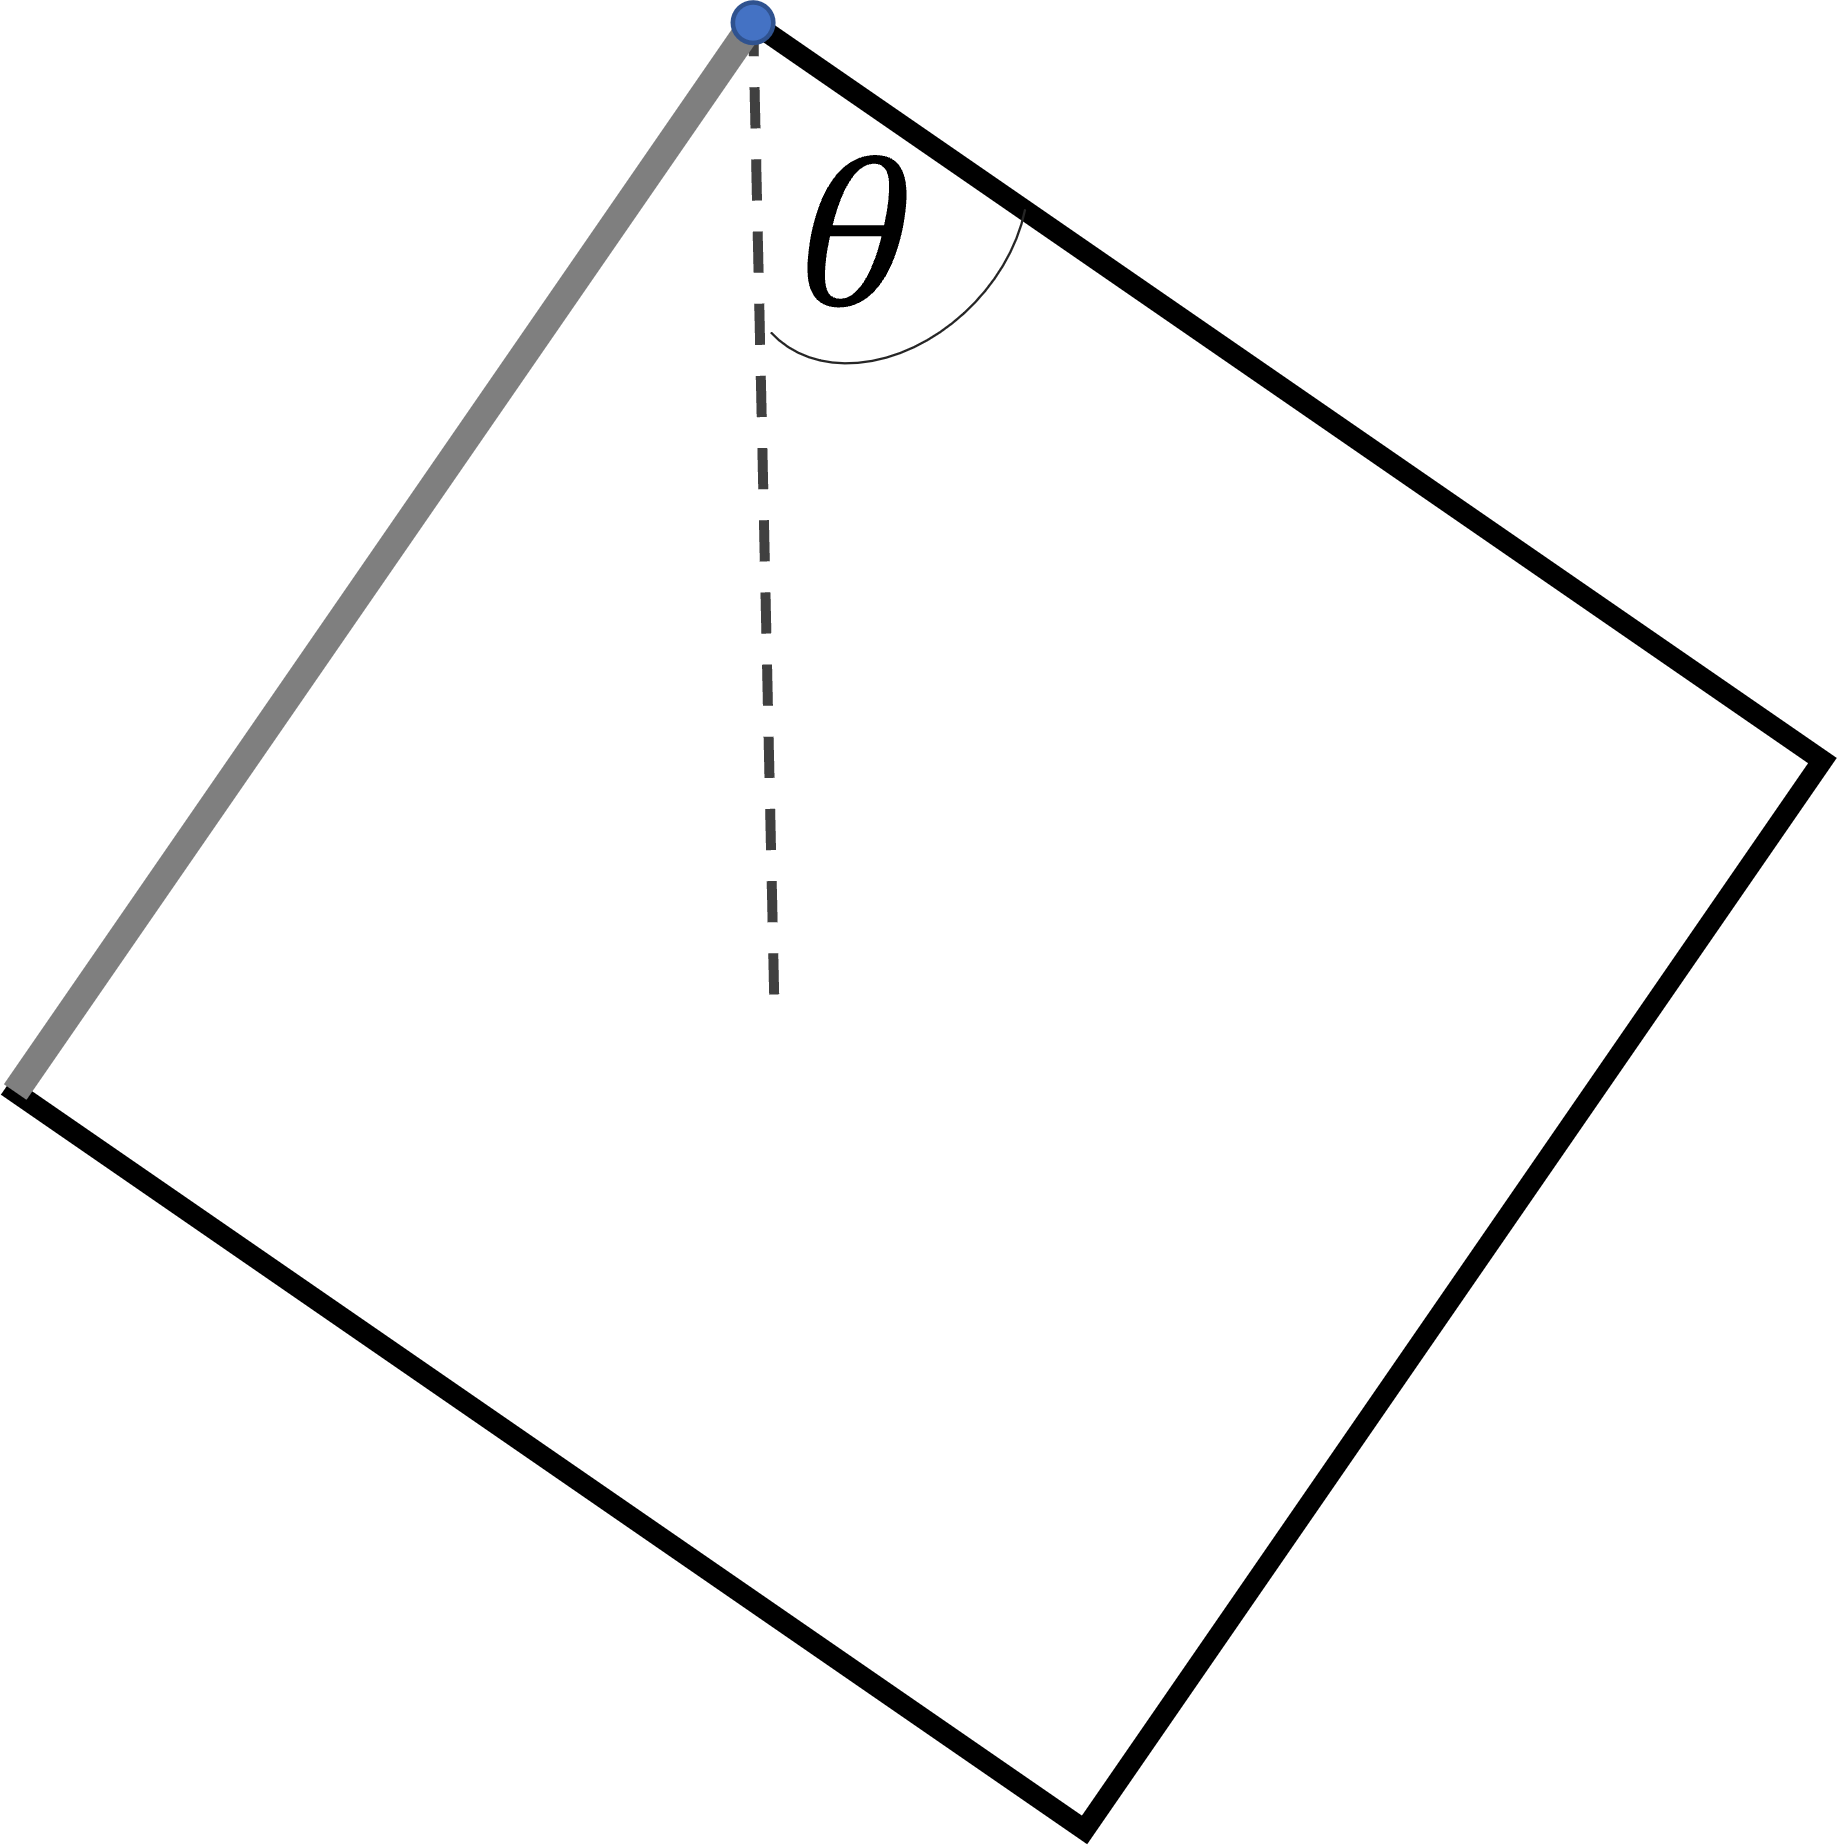
\includegraphics[width=0.7\linewidth]{2022-2/Imagenes/Capsula2/fierro_b.png}
        \caption{}
    \end{subfigure}
\end{figure}




% Para imágenes vectoriales -> el texto tiene que estar en LaTeX
% \begin{figure}[htbp]
%   \centering
%   \svgpath{../Imagenes/ejercicios}  -> .. irse pa'trás 
%   \includesvg{ej5.svg}
% \end{figure}

\end{enumerate}
\end{document}
